\chapter{Аналитическая часть}

\section{Обзор и анализ существующих интернет-магазинов животных}

\hspace{0.6cm} В настоящее время большинство интернет-магазинов позволяют покупать продукцию для животных, узнавать информацию об услугах, имеют удобный и яркий интерфейс. Вот некоторые из них:

\begin{figure}[ht!]
  \centering
  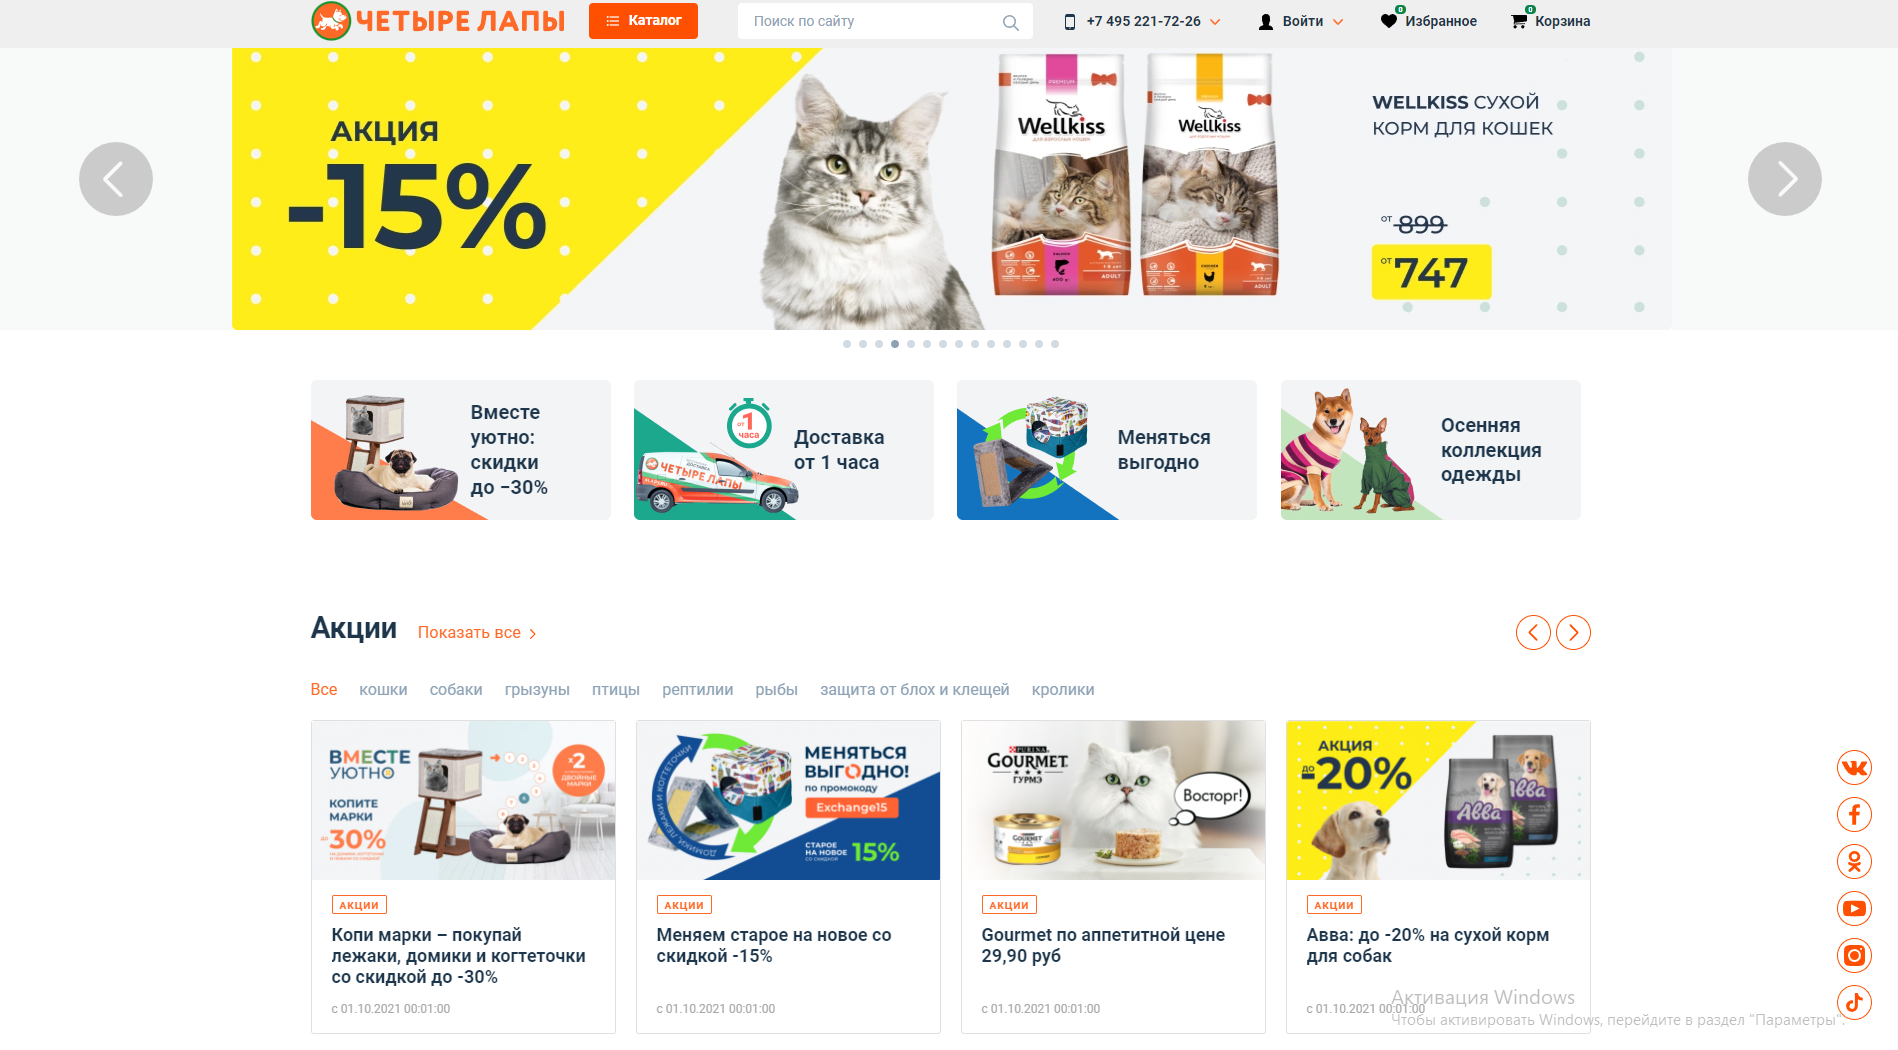
\includegraphics[scale=0.3]{chetirelapy.png}
  \caption{интернет-магазин Четыре Лапы}
  \label{fig:image1}
\end{figure}

\newpage

\begin{figure}[ht!]
  \centering
  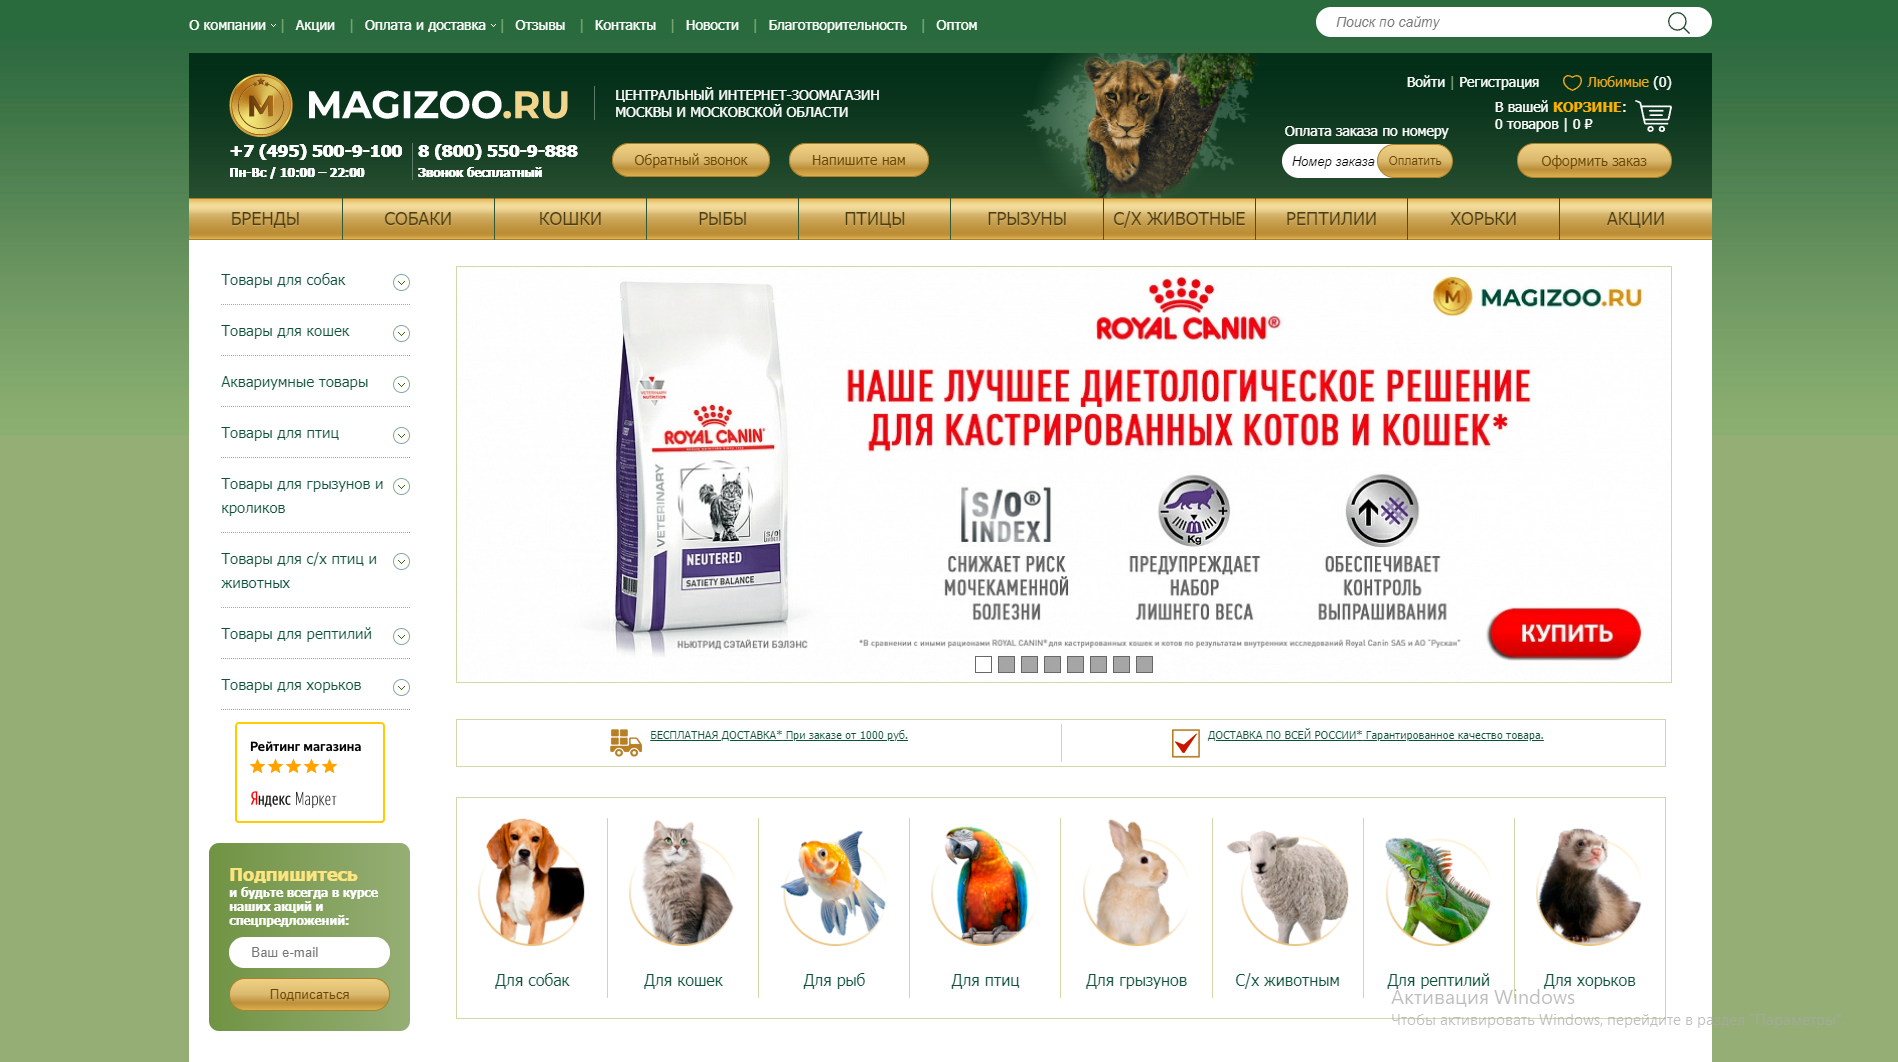
\includegraphics[scale=0.3]{magizoo.png}
  \caption{интернет-магазин Магизу}
  \label{fig:image2}
\end{figure}

\begin{figure}[ht!]
  \centering
  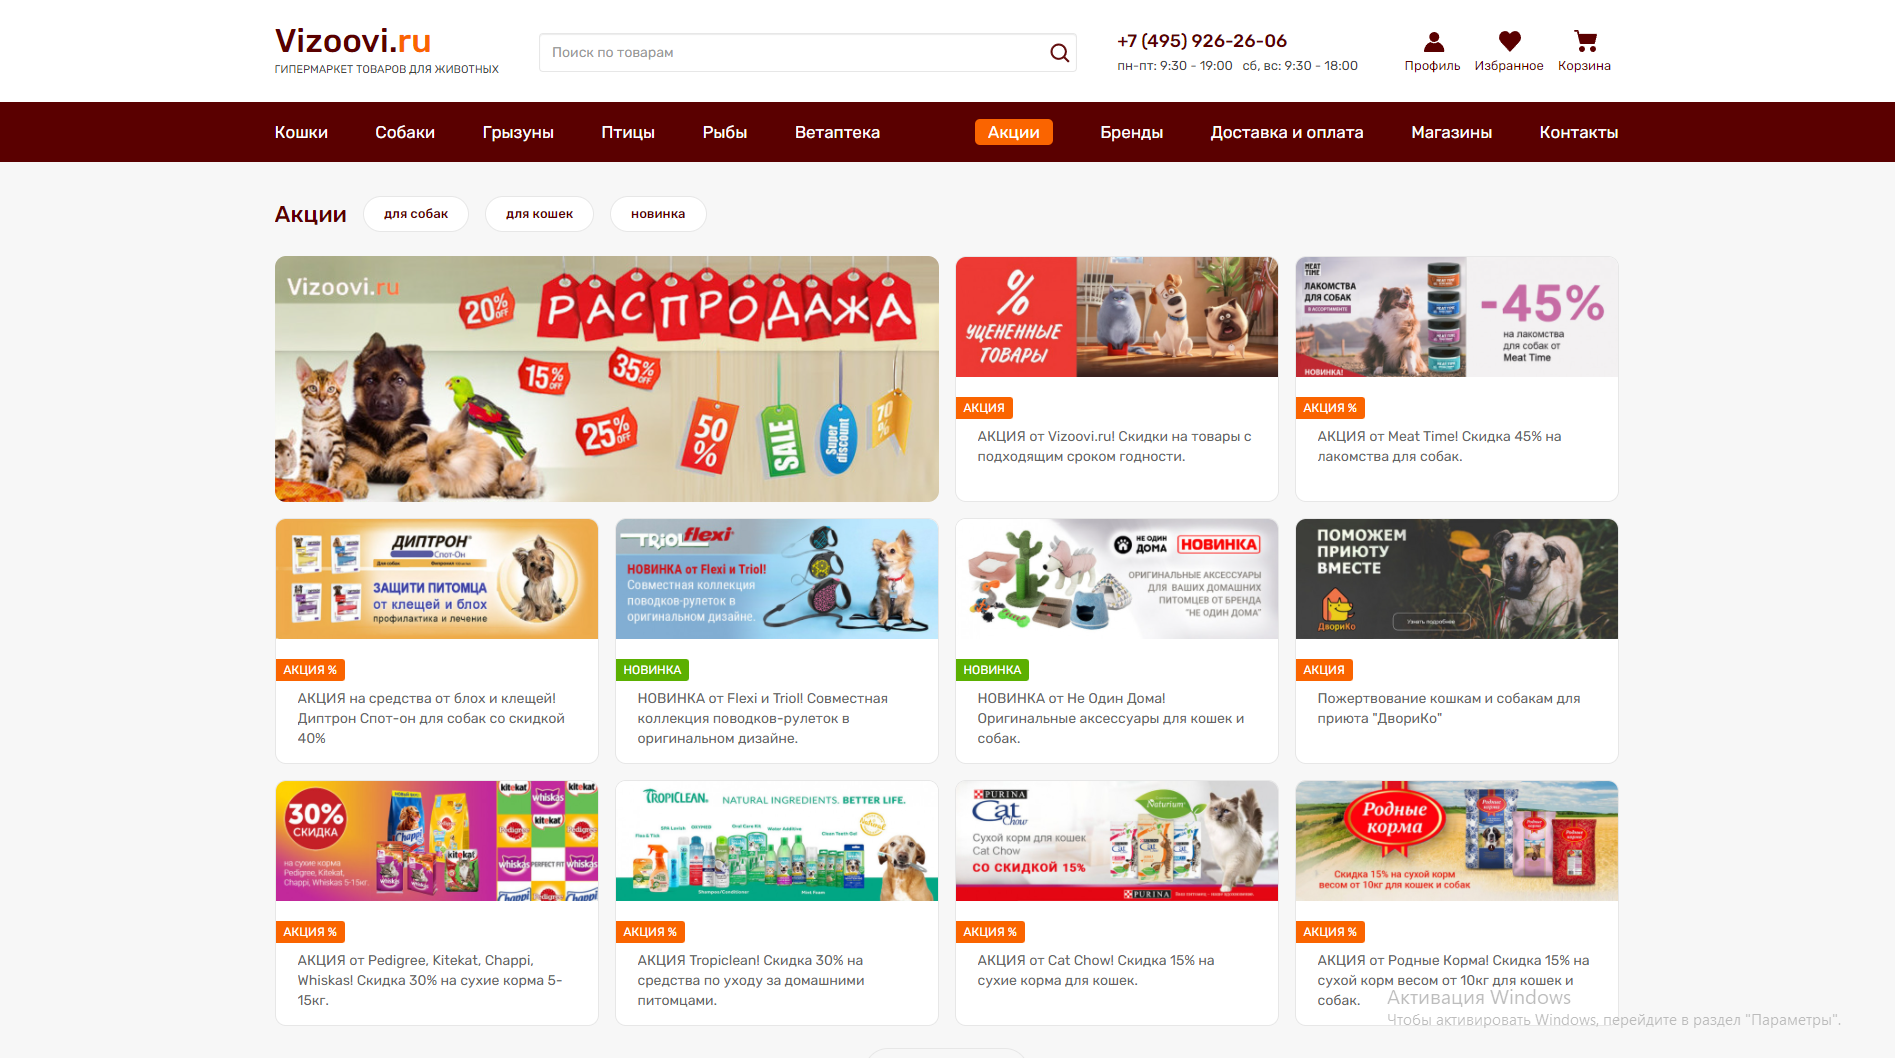
\includegraphics[scale=0.3]{vizoovi.png}
  \caption{интернет-магазин Визуви}
  \label{fig:image3}
\end{figure}

\newpage

\begin{figure}[ht!]
  \centering
  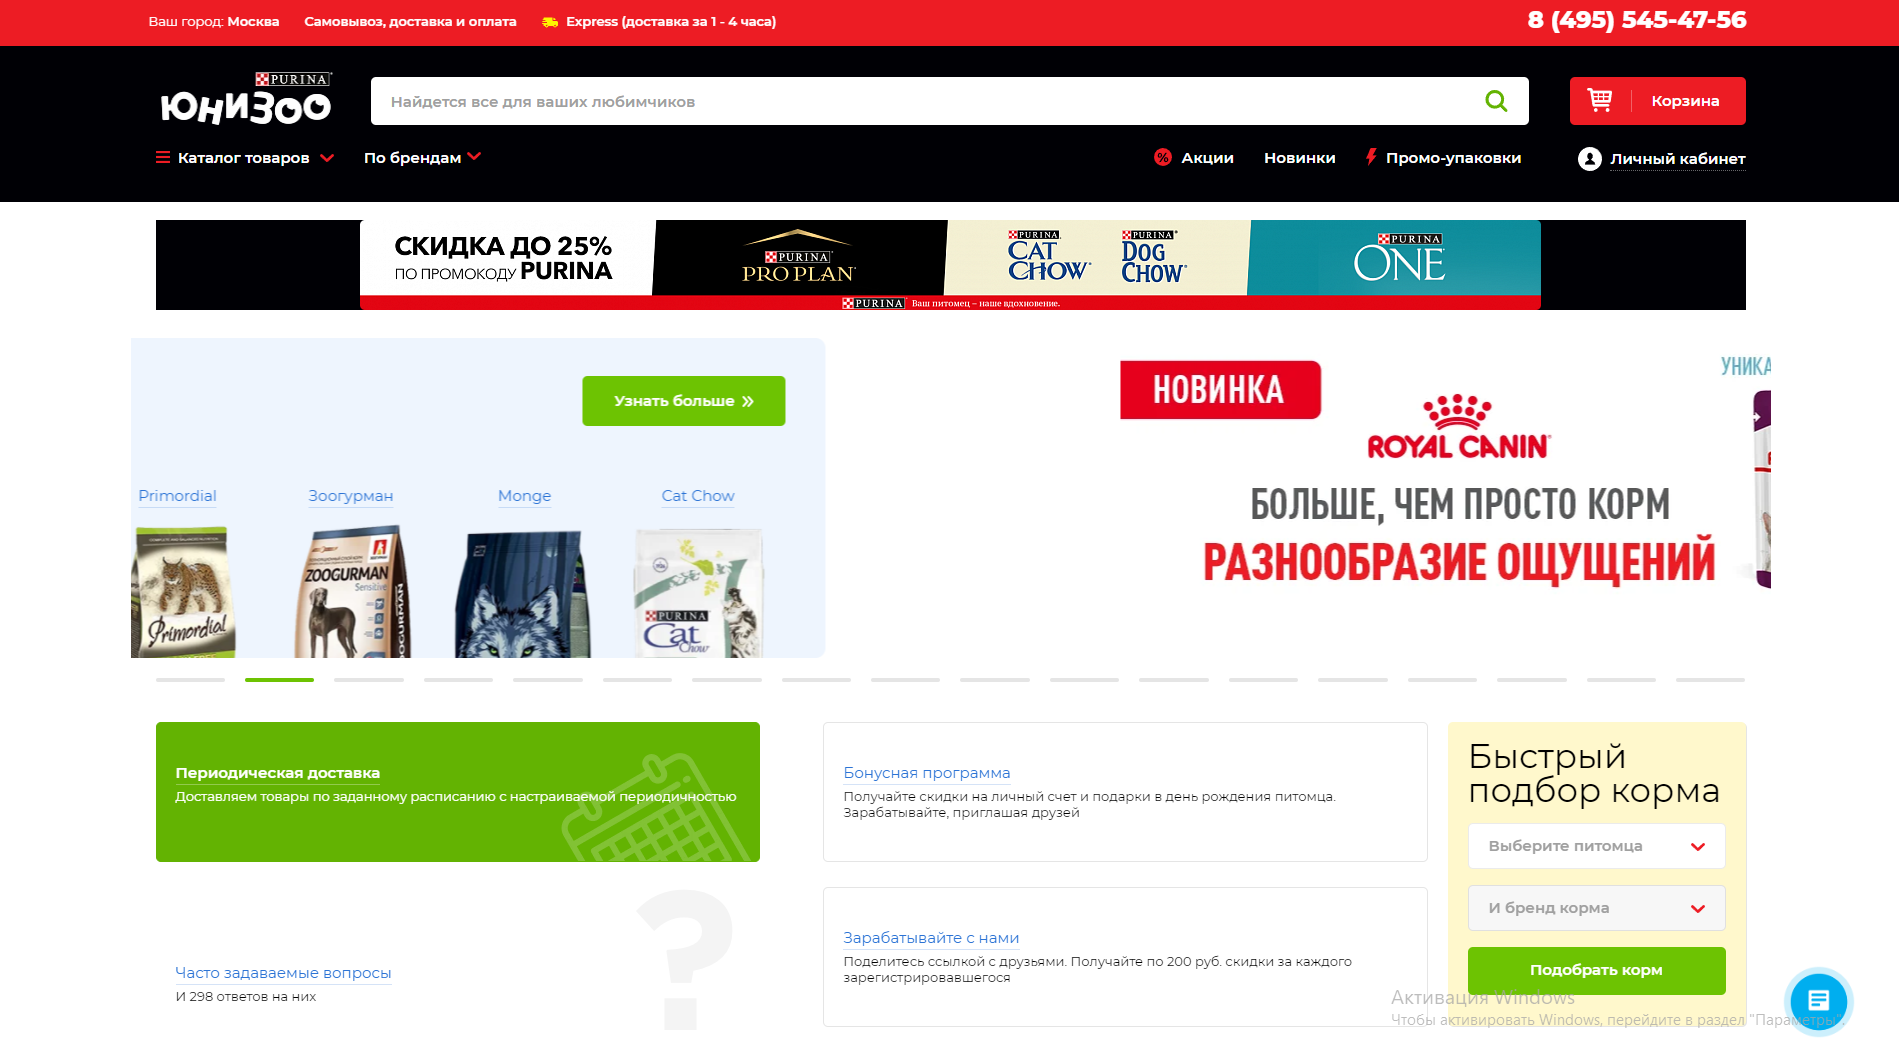
\includegraphics[scale=0.3]{unizoo.png}
  \caption{интернет-магазин Юнизу}
  \label{fig:image4}
\end{figure}

\hspace{0.6cm} Как можно заметить из рисунков \ref{fig:image1}, \ref{fig:image2}, \ref{fig:image3} и \ref{fig:image4}, в основном интерфейс магазинов отличается цветовой гаммой, использованной при создании визуальной составляющей, ассортиментом. Функционал предоставляемый на данных сайтах приблизительно одинаковый. Везде реализованы функции поиска товаров с возможностью фильтровать результат, регистрироваться и авторизоваться на сайте, для того чтобы иметь возможность сделать заказ. Однако в магазинах есть возможность покупать только товары для животных, а функционал предназначен только для покупателей.

\newpage

\hspace{0.6cm} На рисунке \ref{fig:image17} приведена use-case диаграмма, построенная основываясь на функционале приведенных ранее ресурсах. Данная схема составлена с целью отразить логику работы функций, предоставляемых ресурсами.

\begin{figure}[ht!]
  \centering
  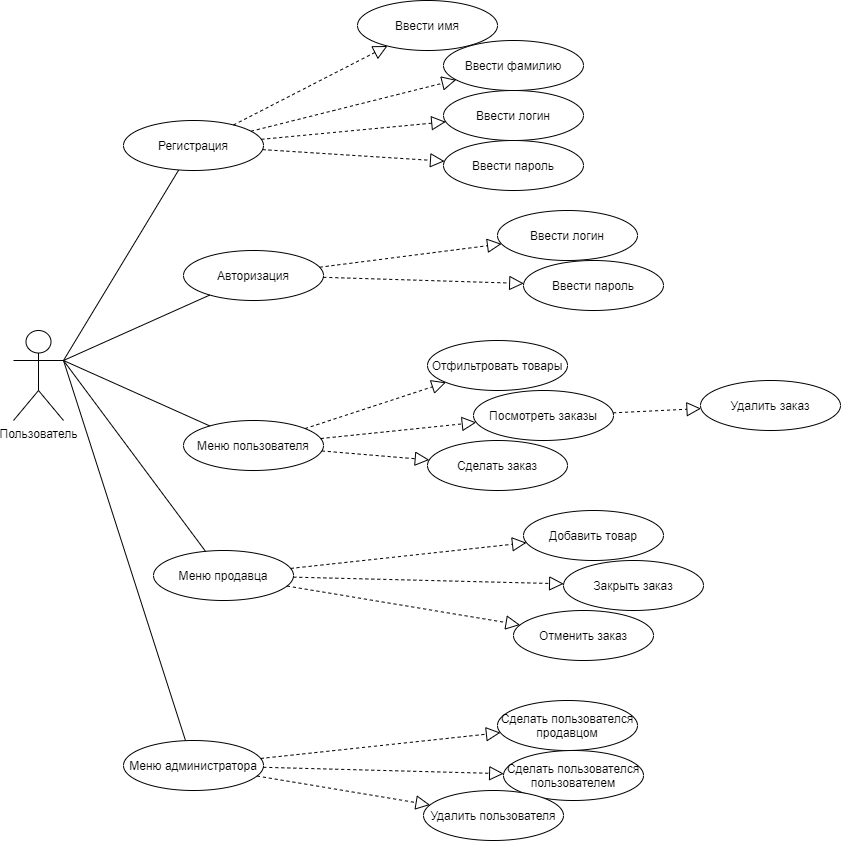
\includegraphics[scale=0.5]{Use-Case диаграмма.drawio.png}
  \caption{Use-Case диаграмма}
  \label{fig:image17}
\end{figure}

\section{Типы баз данных}

\hspace{0.6cm} База данных — это упорядоченный набор структурированной информации или данных, которые обычно хранятся в электронном виде в компьютерной системе. База данных обычно управляется системой управления базами данных (СУБД). Данные вместе с СУБД, а также приложения, которые с ними связаны, называются системой баз данных, или, для краткости, просто базой данных\cite{web:DBTypes}.

\hspace{0.6cm} Существует множество различных типов баз данных. Выбор наилучшей базы данных зависит от того, как и какие данные необходимо использовать.

\subsection{Реляционные базы данных}
Реляционные базы данных стали преобладать в 1980-х годах. Данные в реляционной базе организованы в виде таблиц, состоящих из столбцов и строк. Реляционная СУБД обеспечивает быстрый и эффективный доступ к структурированной информации. На рисунке \ref{fig:image7} приведен пример реляционной БД\cite{web:DBTypes}.

\begin{figure}[ht!]
  \centering
  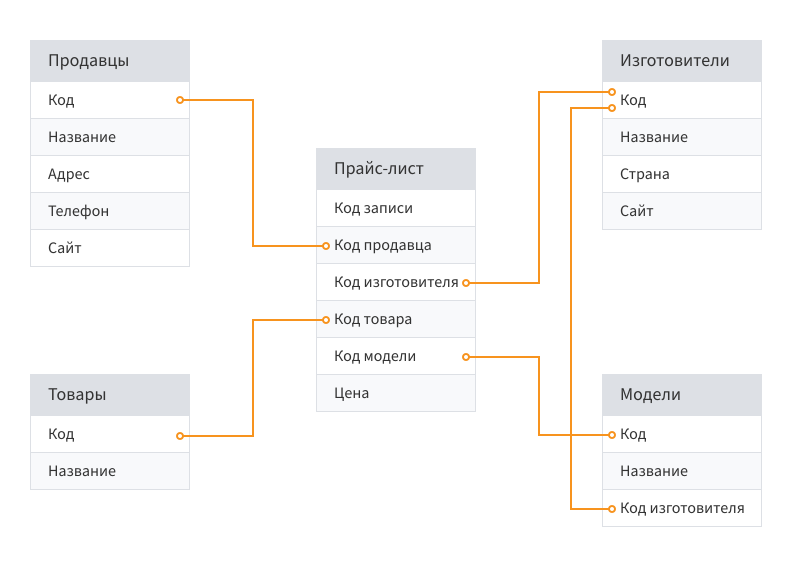
\includegraphics[scale=0.5]{relation-database.png}
  \caption{пример реляционной БД}
  \label{fig:image7}
\end{figure}

\newpage

\hspace{0.6cm} Преимущества:

\begin{itemize}
  \item Простота. В реляционной модели всего одна информационная конструкция, которая формализует табличное представление данных, привычное для пользователей;
  \item Теоретическое обоснование. Наличие теоретически обоснованных методов нормализации отношений позволяет получать БД с заданными характеристиками;
  \item Независимость данных. Когда необходимо изменить структуру реляционной БД, это, как правило, приводит к минимальным изменениям в прикладных программах;
\end{itemize}

\hspace{0.6cm} Недостатки:

\begin{itemize}
  \item Низкая скорость при выполнении операции соединения;
  \item Большой расход памяти для представления реляционной БД;
\end{itemize}

\subsection{Иерархические базы данных}
В Иерархическом типе БД появляются связи между объектами (записями). Каждая запись имеет одного «родителя». Это создаёт древовидную структуру, в которой записи классифицируются по их отношениям с цепочкой родительских записей\cite{web:IerarchiDB}. На рисунке \ref{fig:image12} приведен пример иерархичской бд.

 \begin{figure}[ht!]
  \centering
  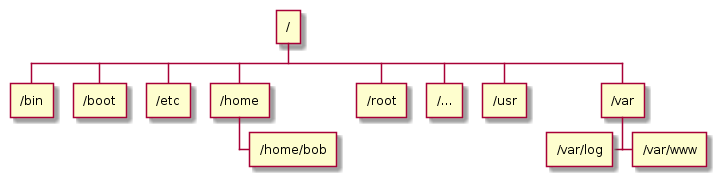
\includegraphics[scale=0.5]{IerarchiDB.png}
  \caption{пример иерархической базы данных}
  \label{fig:image12}
\end{figure}

\hspace{0.6cm} Преимущества:

\begin{itemize}
  \item простота понимания;
  \item простота оценки операционных характеристик.
\end{itemize}

\hspace{0.6cm} Недостатки:

\begin{itemize}
  \item могут быть избыточные данные;
  \item усложняются операции включения и удаления;
  \item удаление исходных объектов ведет к удалению порожденных объектов;
  \item процедурный характер манипулирования данными;
  \item доступ к любому порожденному узлу возможен только через корневой узел;
  \item сильная зависимость логической и физической БД;
  \item сильно ограниченный набор структур запроса.
\end{itemize}

\subsection{Сетевые базы данных}
Сетевые базы данных расширяют функциональность иерархических: записи могут иметь более одного родителя. А значит, можно моделировать сложные отношения. На рисунке \ref{fig:image11} приведен пример сетевой базы данных\cite{web:NetworkDB}.

 \begin{figure}[ht!]
  \centering
  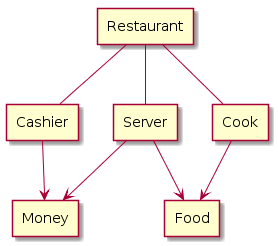
\includegraphics[scale=0.5]{networkDB.png}
  \caption{пример сетевой базы данных}
  \label{fig:image11}
\end{figure}

\hspace{0.6cm} Преимущества:

\begin{itemize}
  \item предоставляет большие возможности в смысле допустимости образования произвольных связей;
\end{itemize}

\hspace{0.6cm} Недостатки:

\begin{itemize}
  \item высокая сложность и жесткость схемы БД, сложность понимания и выполнения обработки информации;
\end{itemize}

\subsection{Графовые базы данных}
Графовая база данных хранит данные в контексте сущностей и связей между сущностями. На рисунке \ref{fig:image10} приведен пример графовой базы данных\cite{web:GraphDB}.

 \begin{figure}[ht!]
  \centering
  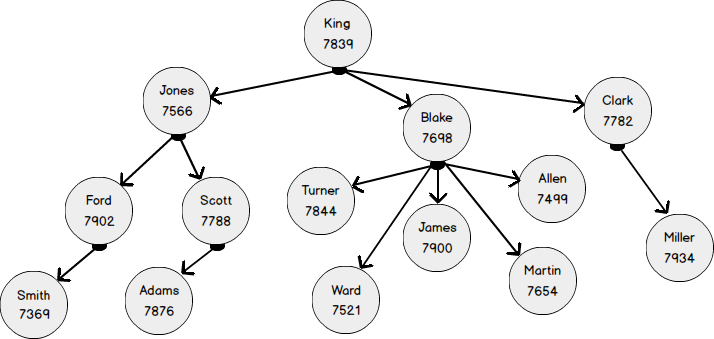
\includegraphics[scale=0.5]{GraphDB.png}
  \caption{пример графовой базы данных}
  \label{fig:image10}
\end{figure}

\hspace{0.6cm} Преимущества:

\begin{itemize}
  \item предоставляют чрезвычайно гибкую модель данных и способ развертывания, соответствующий современным способам развертывания программного обеспечения;
  \item производительность графовых баз данных остается неизменной с увеличением объема хранимых данных.
\end{itemize}

\hspace{0.6cm} Недостатки:

\begin{itemize}
  \item В базе данных графов каждая запись должна проверяться индивидуально во время запроса, чтобы определить структуру данных, в то время как в реляционной базе данных это известно заранее;
  \item база данных использует много места для хранения, потому что нужно хранить все отношения между записями.
\end{itemize}

\section{Выбор реляционных СУБД}

\subsection{SQLite}

\hspace{0.6cm} SQLite - Легко встраиваемая в приложения база данных. Так как это система базируется на файлах, то она предоставляет довольно широкий набор инструментов для работы с ней, по сравнению с сетевыми СУБД. При работе с этой СУБД обращения происходят напрямую к файлам (в эти файлах хранятся данные), вместо портов и сокетов в сетевых СУБД. Именно поэтому SQLite очень быстрая, а также мощная благодаря технологиям обслуживающих библиотек\cite{web:SQLite}.

\hspace{0.6cm} Преимущества:

\begin{itemize}
  \item файловая структура - вся база данных состоит из одного файла, поэтому её очень легко переносить на разные машины;
  \item используемые стандарты - хотя может показаться, что эта СУБД примитивная, но она использует SQL. Некоторые особенности опущены (RIGHT OUTER JOIN или FOR EACH STATEMENT), но основные все-таки поддерживаются;
  \item отличная при разработке и тестировании - в процессе разработки приложений часто появляется необходимость масштабирования. SQLite предлагает всё что необходимо для этих целей, так как состоит всего из одного файла и библиотеки написанной на языке C.
\end{itemize}

\hspace{0.6cm} Недостатки:

\begin{itemize}
  \item отсутствие системы пользователей - более крупные СУБД включают в свой состав системы управления правами доступа пользователей. Обычно применения этой функции не так критично, так как эта СУБД используется в небольших приложениях;
  \item отсутствие возможности увеличения производительности - опять, исходя из проектирования, довольно сложно выжать что-то более производительное из этой СУБД.
\end{itemize}

\subsection{PostgreSQL}

\hspace{0.6cm} PostgreSQL является самым профессиональным из всех трех рассмотренных нами СУБД. Она свободно распространяемая и максимально соответствует стандартам SQL. PostgreSQL или Postgres стараются полностью применять ANSI/ISO SQL стандарты своевременно с выходом новых версий\cite{web:PostgreSQL}.

\hspace{0.6cm} Преимущества:

\begin{itemize}
  \item открытое ПО соответствующее стандарту SQL - PostgreSQL - бесплатное ПО с открытым исходным кодом. Эта СУБД является очень мощной системой;
  \item большое сообщество - существует довольно большое сообщество в котором вы запросто найдёте ответы на свои вопросы;
  \item большое количество дополнений - несмотря на огромное количество встроенных функций, существует очень много дополнений, позволяющих разрабатывать данные для этой СУБД и управлять ими;
  \item расширения - существует возможность расширения функционала за счет сохранения своих процедур;
  \item объектность - PostrgreSQL это не только реляционная СУБД, но также и объектно-ориентированная с поддержкой наследования и много другого.
\end{itemize}

\hspace{0.6cm} Недостатки:

\begin{itemize}
  \item производительность - при простых операциях чтения PostgreSQL может значительно замедлить сервер и быть медленнее своих конкурентов, таких как MySQL;
  \item популярность - по своей природе, популярностью эта СУБД похвастаться не может, хотя и присутствует довольно большое сообщество;
  \item хостинг - в силу выше перечисленных факторов иногда довольно сложно найти хостинг с поддержкой этой СУБД.
\end{itemize}

\subsection{MySQL}

\hspace{0.6cm} MySQL - это самая распространенная полноценная серверная СУБД. MySQL очень функциональная, свободно распространяемая СУБД, которая успешно работает с различными сайтами и веб приложениями. Обучиться использованию этой СУБД довольно просто, так как на просторах интернета вы легко найдете большее количество информации\cite{web:SQLite}.

\hspace{0.6cm} Преимущества:

\begin{itemize}
  \item простота в работе - установить MySQL довольно просто. Дополнительные приложения, например GUI, позволяет довольно легко работать с БД;
  \item богатый функционал - MySQL поддерживает большинство функционала SQL;
  \item безопасность - большое количество функций обеспечивающих безопасность, которые поддерживается по умолчанию;
  \item масштабируемость - MySQL легко работает с большими объемами данных и легко масштабируется;
  \item скорость - упрощение некоторых стандартов позволяет MySQL значительно увеличить производительность.
\end{itemize}

\hspace{0.6cm} Недостатки:

\begin{itemize}
  \item известные ограничения - по задумке в MySQL заложены некоторые ограничения функционала, которые иногда необходимы в особо требовательных приложениях;
  \item проблемы с надежностью - из-за некоторых способов обработки данных MySQL (связи, транзакции, аудиты) иногда уступает другим СУБД по надежности;
  \item медленная разработка - Хотя MySQL технически открытое ПО, существуют жалобы на процесс разработки. Стоит заметить, что существуют другие довольно успешные СУБД созданные на базе MySQL, например MariaDB.
\end{itemize}

\subsection{MariaDB}

\hspace{0.6cm} MariaDB – это по-настоящему открытый дистрибутив MySQL (выпущен под GNU GPLv2). Он был создан после приобретения Oracle MySQL, когда некоторые из основных разработчиков MySQL были обеспокоены тем, что Oracle подорвет его философию открытого исходного кода.

\hspace{0.6cm} MariaDB был разработан, чтобы быть максимально совместимым с MySQL при замене нескольких ключевых компонентов. Он использует механизм хранения Aria, который функционирует как транзакционный, так и нетранзакционный механизм. Некоторые даже предполагали, что Aria станет стандартным движком для MySQL в будущих выпусках, прежде чем MariaDB станет независимым проектом\cite{web:MariaDB}.

\hspace{0.6cm} Преимущества:

\begin{itemize}
  \item многие пользователи выбирают MariaDB вместо MySQL из-за частых обновлений систем безопасности MariaDB. Хотя это не обязательно означает, что MariaDB более безопасна, это означает, что сообщество разработчиков серьезно относится к безопасности;
  \item другие говорят, что основные преимущества MariaDB в том, что она почти наверняка останется с открытым исходным кодом и будет полностью совместима с MySQL. Это означает, что миграция из одной системы в другую происходит очень быстро;
  \item благодаря этой совместимости MariaDB также хорошо работает со многими другими языками, которые обычно используются в MySQL. Это означает, что на изучение и отладку кода тратится меньше времени;
  \item можно установить и запустить WordPress с MariaDB вместо MySQL для лучшей производительности и более богатого набора функций. WordPress является самой популярной CMS от markethare, которая обеспечивает почти половину контента в интернете, и имеет активное сообщество разработчиков с открытым исходным кодом. Сторонние темы и плагины работают так, как задумано, когда WordPress установлен с MariaDB.
\end{itemize}

\hspace{0.6cm} Недостатки:

\begin{itemize}
  \item MariaDB несколько подвержен «вздутию живота». Его центральный файл журнала IDX, в частности, имеет тенденцию становиться очень большим после длительного использования, что в конечном итоге снижает производительность;
  \item кэширование – это еще одна область, в которой MariaDB могла бы усовершенствоваться. Этот процесс не такой быстрый, каким мог бы быть, что немного расстраивает;
  \item несмотря на все первоначальные обещания, MariaDB больше не полностью совместима с MySQL. Если вы переходите с MySQL, вам нужно будет выполнить перекодировку.
\end{itemize}

\newpage

\section{Вывод}

\hspace{0.6cm} Проанализировав существующие ресурсы для покупки питомцев, было решено создать веб-приложение, в котором будет реализован функционал представленный в ресурсах, а также функционал для продавцов, с возможностью обрабатывать заказы и администратора, для осуществления контроля за продавцами и покупателями. На основании анализа предметной области была построена ER-диаграмма, продемонстрированная на рисунке \ref{fig:image16}.

 \begin{figure}[ht!]
  \centering
  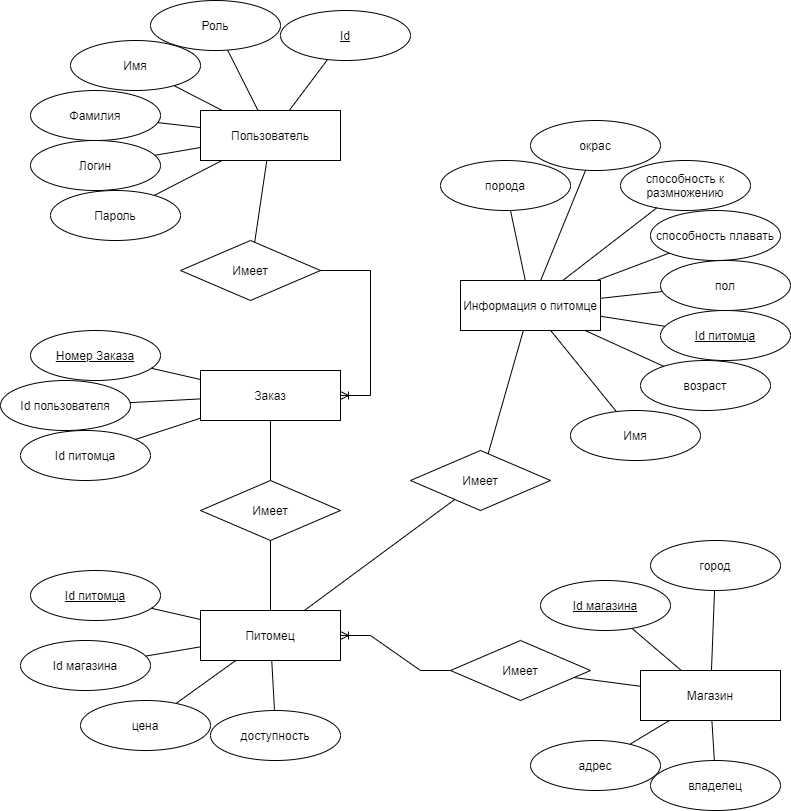
\includegraphics[scale=0.5]{ER-модель.drawio.png}
  \caption{ER-диаграмма}
  \label{fig:image16}
\end{figure}

\newpage

\hspace{0.6cm} Проанализировав все варианты типов БД, было решено выбрать реляционную базу данных и работать с СУБД MySQL. Достоинства данной модели:

\begin{itemize}
  \item простота в работе - установить MySQL довольно просто. Дополнительные приложения, например GUI, позволяет довольно легко работать с БД;
  \item богатый функционал - MySQL поддерживает большинство функционала SQL;
  \item безопасность - большое количество функций обеспечивающих безопасность, которые поддерживается по умолчанию;
  \item масштабируемость - MySQL легко работает с большими объемами данных и легко масштабируется;
  \item скорость - упрощение некоторых стандартов позволяет MySQL значительно увеличить производительность.
\end{itemize}



